\documentclass[12pt]{amsart}
\usepackage{mathrsfs}
\usepackage{amsmath}
\usepackage{amssymb}
\usepackage{amsfonts}
\usepackage{amsopn}
\usepackage{amsthm}
\usepackage{latexsym}
\usepackage[all]{xy}
\usepackage{enumerate}
\usepackage{geometry}
%\usepackage{biblatex}
%\usepackage{hyperref}
%\usepackage[autostyle]{csquotes}
\usepackage{fancyhdr}
\usepackage{graphicx}
\usepackage{wrapfig}
\usepackage{float}

\usepackage[
    backend=biber,
style=alphabetic,
sorting=nyt,
bibencoding=utf8,
   % style=authoryear-icomp,
    %sortlocale=de_DE,
    %natbib=true,
    %author=true,
%style=verbose,
%journal=true,
%url=true, 
%    doi=false,
%    eprint=true
]{biblatex}
\addbibresource{STABLEreferencesX.bib}

\usepackage[]{hyperref}
\hypersetup{
    colorlinks=true,
}


\newtheorem{thm}{Theorem}
\newtheorem{lem}[thm]{Lemma}
\newtheorem{prop}[thm]{Proposition}
\newtheorem*{prob}{Problem}
\newtheorem{cor}[thm]{Corollary}
\newtheorem{question}[thm]{Question}
\newtheorem*{hyp}{Hypothesis}
\theoremstyle{definition}
\newtheorem{dfn}[thm]{Definition}
\newtheorem{exx}[thm]{Example}
\theoremstyle{remark}
\newtheorem{rem}[thm]{Remark}
\newcommand{\fh}{\mathfrak{h}}
\newcommand{\bn}{\mathbf{n}}
\newcommand{\bC}{\mathbb{C}}
\newcommand{\bG}{\mathbb{G}}
\newcommand{\bR}{\mathbb{R}}
\newcommand{\fB}{\mathfrak{B}}
\newcommand{\bZ}{\mathbb{Z}}
\newcommand{\bQ}{\mathbb{Q}}
\newcommand{\bq}{\bar{Q}[t]}
\newcommand{\bb}{\bullet}
\newcommand{\del}{\partial}
\newcommand{\sB}{\mathscr{B}}
\newcommand{\sE}{\mathscr{E}}
\newcommand{\mR}{\bR^\times_{>0}}
\newcommand{\hh}{\hookleftarrow}
\newcommand{\bD}{\mathbb{D}}
\newcommand{\Gm}{\mathbb{G}_m}
\newcommand{\uF}{\underline{F}}
\newcommand{\sC}{\mathscr{C}}
\newcommand{\bX}{\overline{X}^{BS/\bQ}}
\newcommand{\sT}{\mathscr{T}}
\newcommand{\sW}{\mathscr{W}}
\newcommand{\sZ}{\mathscr{Z}}

\begin{document}

\title{Closing Steinberg Symbols of the Mapping Class Group: Open Questions}
\author{J. H. Martel}
\date{\today}
\email{jhmartel@protonmail.com}
\maketitle

\begin{abstract}
This article studies an algebraic problem which we call Closing the Steinbeg symbol (CS) of the mapping class group of compact Riemann surfaces $\Sigma = \Sigma_g$. For concreteness we focus on the genus two ($g=2$) case. Formally solving (CS) requires finding finite subsets $I$ of $\Gamma:=MCG(\Sigma)$ such that the translates $\sum_{\gamma \in I}\sB.\gamma$ of a certain chain sum $\sB:=\sum_i \alpha_i$ is a nontrivial homology cycle, see \ref{CS} for details. Solutions $I$ to (CS) which satisfy additional convexity assumptions \eqref{cs} lead to our producing candidate equivariant deformation retracts $\sT_g \leadsto \sZ$ of the Teichmueller space $\sT_g$ onto a subvariety $\sZ$. The construction of these retracts and the subvariety $\sZ$ is based on the Reduction to Singularity methods of the author's thesis \cite{martel}. 
\end{abstract}


\tableofcontents




%The subvariety $\sZ=\sZ_\pi$ is a closed subset of the singularity locus of an optimal semicoupling $\pi=\pi(c,\sigma, \tau)$ with respect to a source $\sigma$, target $\tau$, and cost $c$ of transporting unit source to unit target mass. Positive solutions of (CS) lead to candidate equivariant spines $\sZ$ of $\sT$ based on the Reduction-to-Singularity method of the author's thesis \cite{martel}. The deformation retracts are constructed by an auxiliary function $\eta_{avg}(x,y_0, y_1)$ representing an averaged interaction potential. [INCOMPLETE]

%The bridge from solutions to (CS) to deformation retracts $\sT_g \leadsto \sZ$ is based on the ``reduction to singularity" methods of the author's thesis \cite{martel}, where we show the homotopy type of $\sZ$ is determined by an analytic criteron which we call Uniform Halfspace Condition (UHS). This requires an averaged vector potential denoted $\eta_{avg}(x,y_0,y_1)$ to be bounded away from zero uniformly with the target variables. Verifying (UHS) is a computational problem, and beyond the scope of this present article. The present article concludes with a question to [ref] concerning further computational problems in genus $g=2$.



%In general the retracts $\sZ$ are /`a priori of positive codimension $(>0)$. 

%And equivariant retracts onto codimension one hypersurfaces is widely known in literature [ref]. But our method can readily produce larger codimension, even $codim_{\sT} \sZ > > 2$ when the target $\tau$ exhibits sufficient symmetries. 


\section{MCG and Bieri-Eckmann Duality}

Let $\Sigma_g$ be a closed hyperbolic surface genus $g \geq 2$, and let $\Gamma:=MCG(\Sigma_g)$ be the mapping class group of orientation preserving diffeomorphisms. According to topologists, we have $MCG(\Sigma)=\pi_0(Diff_+(\Sigma))$ which is the group of  orientation preserving automorphisms of $\Sigma$ modulo isotopy. According to algebraists, we have also Dehn-Neilsen-Baer's identification $MCG(\Sigma)=Out(\pi_1(\Sigma))$, where $\pi_1(\Sigma)=\pi_1(\Sigma, pt)$ is Poincar\'e's pointed fundamental group. %See [ref] for proofs. %For computations we find neither representation sufficiently effective, e.g. [ss]. 




%However the results described apply more generally to discrete groups $\Gamma$ which satisfy Bieri-Eckmann's homological duality and having finite virtual cohomological dimension. [Ref].

%[Intro]
%This article studies some homological properties of $\Gamma$, and their relation to constructing small dimensional $E\Gamma$ models (so called ``spines"). Specifically we introduce a problem called ``Closing the Steinberg symbol" and explain its application to constructing spines. The basic ideas were developed in our PhD thesis [ref].

%Naively, it's clear from experience that precise fundamental domains (precise reduction theory) is essentially an intractable problem. Moreover it's not clear that a precise fundamental domain is even desirable, or useful, in constructing spines. Our thesis [ref] introduces a general method of ``reduction to singularity", by which spines are represented as the singularity locus of an optimal transportation. We elaborate below.

The group-theoretic (co)homology of $\Gamma$ is defined via the symmetries of proper discontinuous actions $X\times \Gamma \to X$ on $E\Gamma$ models $X$. There is extensive literature on the subject, basic introductions include \cite{Brown}. The standard $E\Gamma$ model for the mapping class (modular) group of closed orientable Riemann surfaces is Teichmueller's $X=\sT_g$, a topological $(6g-6)$-cell $\simeq \bR^{6g-6}$, e.g. \cite{hubbard}. There are alternative models which are also worth exploring, as will be discussed below (\S \ref{s2}).

%There is further a canonical uniform source measure on $\sT_g$

It is a fundamental observation of Harvey \cite{Harvey}, Ivanov \cite{ivanov2015virtual}, Harer \cite{Harer1986}, etc., that $\Gamma=MCG(\Sigma_g)$ is a Bieri-Eckmann virtual duality group \cite{BiEck}, where a key role is played by the action of $\Gamma$ on the simplicial curve complex $\sC$ and its reduced singular homology and chain groups. The problem of (CS) is based on homological properties of $\Gamma$, and specifically a representation of Bieri-Eckmann's dualizing module $\bD$ with the reduced homology of an excision boundary $\bD\simeq \tilde{H}_*(\del \sT[t]; \bZ)$, where $\sT[t]$ is a maximal $\Gamma$-rational excision of Teichmueller space. See section [ss] below.

For the formalists, we present some definitions below.
\begin{dfn} 
A finitely generated group $\Gamma$ is a duality group of dimension $\nu \geq 0$ with respect to a $\bZ \Gamma$-module $\bD$, if there exists an element $[B]\in H_\nu(\Gamma; \bD)$ with the following property: for every $\bZ \Gamma$-module $A$, the ``cap-product with $[e]$" defines $\bZ \Gamma$-module isomorphisms $H^d(\Gamma;A) \approx H_{\nu-d}(\Gamma; A \otimes \bD)$, $f\mapsto f\cap [e]$. 
\end{dfn}

The basic properties of duality groups are summarized in the following
\begin{prop}[Bieri-Eckmann duality, \cite{BiEck}] \label{dual1}
Let $\Gamma$ be duality group of dimension $\nu$, with dualizing module $\bD$. Then 

(i) we have $\bZ \Gamma$-isomorphism $\bD \approx H^\nu(\Gamma;\bZ \Gamma) \neq 0$, so $\bD$ is a torsion-free additive abelian group;

%\item[(ii)] the dualizing module $D$ is finitely-generated $\bZ\Gamma$-module;

(ii) the homology group $H_\nu (\Gamma; \bD)$ is infinite cyclic generated by $[e]$ as additive abelian group; 

(iii) the group $\Gamma$ has cohomological dimension $cd(\Gamma)$ equal to $\nu$.
\end{prop}


\begin{proof} 
The statements are direct consequences of duality. (i) We see $H^\nu(\Gamma; \bZ \Gamma)$ $\approx H_0(\Gamma; \textbf{D})\approx \textbf{D}$. (ii) Duality implies $H^0(\Gamma; \underline{\bZ} )$ is isomorphic to $H_\nu(\Gamma; \underline{\bZ} \otimes_{\bZ \Gamma} \textbf{D})$, which in turn is canonically isomorphic to $H_\nu(\Gamma; \textbf{D})$ since $\underline{\bZ}\otimes_{\bZ \Gamma} \bZ \Gamma$ $\approx \textbf{D}$. But $H^0(\Gamma, \underline{\bZ})$ is canonically isomorphic to $\underline{\bZ}$. (iii) The duality isomorphism implies for every $\bZ \Gamma$-module $A$ that $H^*(\Gamma; A)$ is isomorphic to $H_{\nu-*}(\Gamma; A \otimes \textbf{D})$ which reduces to $0$ whenever $\nu-*<0$.
\end{proof}

Most importantly, for the mapping class group $\Gamma$, the dualizing module $\bD$ can be identified with the reduced homology of the simplicial curve complex: that is, we can identify $\bD$ up to $\bZ\Gamma$-isomorphism as $\bD=\tilde{H}_*(\sC;\bZ)$, where of course the reduced homology group inherits the natural structure of $\bZ \Gamma$-module from the action of $\Gamma$ on $\sC$. The curve complex has the homotopy-type of a countable bouquet of $(2g-2)$-dimensional spheres, c.f. \cite{ivanov2015virtual}, \cite{Harer1986}. Thus we deduce that $$vcd(\Gamma)=6g-6-(2g-2)+1=4g-5.$$ For example, this implies the Teichmueller space of genus two closed surfaces is (modulo mapping class group) a $6$-dimensional manifold, yet having the algebraic topology of a $3$-dimensional complex.  


\section{Canonical Riemannian metrics on $\sT_g$ and Flat Filling}\label{s2}

Teichmueller's theorem that $\sT_g$ is a $(6g-6)$-dimensional cell is perhaps misleading because the $\Gamma$-equivariant topology of $\sT_g$ is highly nontrivial, and only locally resembling a $(6g-6)$ cell. The construction of $\Gamma$ equivariant metrics $d$ on $\sT$ is non canonical and there are many candidates. Popular metrics are Teichmueller's original metric $d_{Teich}$ \cite{hubbard},  Weil-Peterson's metric $d_{WP}$ \cite{hubbard}, Thurston's metric \cite{wolpert1986a}, or McMullen's \cite{mcmullen2000moduli}. 

For a choice of invariant Riemannian metric $d$ on $\sT$ and invariant function $t: \sC^0 \to \bR_{>0}$, we define an excision $\sT[t]$ of $\sT$ by excising (``scooping out") convex horoballs centred at various points at infinity. Our method distinguishes the $\Gamma$-rational horoball excisions which enjoy the further property of having $\Gamma$-invariant boundary horospheres. Thus $\Gamma$ acts proper discontinuously on both $\sT[t]$ and $\del \sT[t]$. We further emphasize those parameters $t$ which are sufficiently small, in which case the excisions $\sT[t]$  have a $\Gamma$-equivariant topological boundary $\del \sT[t]$ with the homotopy-type of $\sC$. This important fact implies a canonical isomorphism $$\bD\approx \tilde{H}_*(\del \sT[t]; \bZ).$$ For the constructive topologist the $\Gamma$-action on $\sT$ is more accesible than the abstract algebraic action on $\bD$. The homologically essential spheres of $\sC$ can be viewed as spheres at-infinity within the excision $\sT[t]$. The $\Gamma$-orbit of these spheres and their singular chain sums generates an important topological $\bZ \Gamma$-module called the \emph{Steinberg module}. Following convention we designate the generator of this module a Steinberg symbol $B$, c.f. ``modular symbols" in \cite{AR}, \cite{AGM}, \cite{Stein}, \cite{Sol}, and references therein. 

The contractibility of $\sT[t]$, $\sT$, and the long exact sequence in relative homology implies the natural boundary morphism $$\delta: C_*(\sT[t], \del \sT[t]) \to C_{*-1}(\del \sT[t])$$ is an isomorphism. Here $C_*$ denotes the singular chain groups. However what we require for applications is an inverse operation which is well-defined directly on singular chains, namely $$FILL:=\delta^{-1}: C_{*-1}(\del \sT[t]) \to C_*(\sT[t], \del \sT[t])$$. This inverse operation is a \emph{filling} operation and requires a choice of metric $d'$. For our applications, any metric $d'$ with the following properties would be desirable:
\begin{itemize}
\item[(M1)] the metric $d'$ is metrically complete and proper in the interior of $\sT$;
\item[(M2)] the metric has nonpositive sectional curvature $(\kappa \leq 0)$ in $\sT$;
\item[(M3)] the $(2g-2)$-dimensional spheres generating the Steinberg symbol at infinity admits a unique $d'$-flat filling $(\kappa =0)$ to relative cycles in $(\sT[t], \del \sT[t])$.
\end{itemize}

If we examine the usual metrics, we find the WP metric has properties (M1), (M2). The author does not know if (M3) holds, although \cite{FarbRank} appears to suggest otherwise. We observe that (M2) has the important consequence that WP-horoballs are geodesically convex in $(\sT, d_{WP})$, \cite{GroCurv}. 

With respect to Teichmuller's original metric, we know (a) holds, but (b) fails and Teichmueller's original metric has regions of positive curvature. Moreover recent work of \cite{RafiBourque} shows that ``convex hull" constructions are not possible in Teichmueller's metric.

When (M3) holds, the Steinberg symbol $B$ canonically fills to a flat relative cycle $(P, \del P)$ in $(\sT[t], \del \sT[t])$, and we call the flat relative cycles $P=FILL[B]$ ``panels". The motivation for the terminology is given in \S \eqref{CS} below. The panels are homologically nontrivial relative cycles in $\sT[t]$ modulo the boundary $\del \sT[t]$. The reduction to singularity method of \cite{martel} does not strictly need flatness in property (M3) -- what is essential is rather the \emph{geometric uniqueness} of such fillings. Any metric $d'$ satisfying the properties (M123) on $\sT$ would readily lead to the existence of equivariant homotopy reductions of $\sT$ onto a candidate spine $\sZ$ according to \cite{martel}. 


The following is very important lemma for our method:

\begin{lem}\label{kl}
Let $d'$ be a metric on $\sT$ satisfying properties $(M123)$. Let $\sT[t]$ be a maximal $\Gamma$-rational excision with sufficiently small parameter $t$. Let $B$ be a Steinberg symbol, and $P=FILL[B]$ the flat-filling. Then $P$ has zero geometric self-intersection in the quotient $\sT[t]/\Gamma$.
\end{lem}
\begin{proof}

\end{proof}

To motivate Lemma \ref{kl}, recall the familiar fact that if $\Sigma$ is a closed hyperbolic surface, and $\alpha$ is a closed geodesic on $\Sigma$, then the lifts $\tilde{\alpha}$ of $\alpha$ to the universal covering $\tilde{\Sigma}$ form a $\pi_1(\Sigma)$ orbit in $\tilde{\Sigma}$ where all the translates are disjoint. Likewise Lemma \ref{kl} asserts that the $\Gamma$-translates of $P$ are disjoint in the interior of $\sT[t]$, and the quotient $\sT[t] \to \sT[t]/\Gamma$ maps $P$ isometrically onto its image.

The existence of parabolic elements $\gamma$ in $\Gamma$ on the other hand, shows that asymptotically as $t\to 0^+$ the relative cycle $P$ and its translates $P.\gamma$ have intersections ``at infinity". However with respect to an equivariant rational parameter $t$, there is no self intersection in the \emph{interior} of $\sT[t]$.

%Wolpert [ref] has important formulas describing gradients of WP distance function. 

%Thus the property (b) in [ss] is crucial, as we follow Gromov's ``filling" arguments from [ref: VBC].




\section{Closing Steinberg}\label{CS}
The problem of Closing Steinberg is informally related to stitching a closed football $F$ from a sequence of panels $\{P_i\}_{i\in I}$. The panels $P_i$ are required to have the property that $F=conv\{P_i|~i\in I\}$ and such that $\sum_{i\in I} \del P_i=0$ over $\bZ/2\bZ$-coefficients. In otherwords, the problem requires finding a sequence of panels $P_i, i\in I$ which assemble to a closed compact convex subset $F$ as defined above. The panels $P=P_i$ of the above footballs are analogous to the flat-filled Steinberg symbols $P=FILL[B]$ and their translates $B.\gamma$, $\gamma\in \Gamma$. Compare Figure \ref{nikeball}.

 %where $\bD:=\tilde{H}_\nu (\sT[t]; \del \sT[t])$ is the reduced singular homology group of the excision model $\sT[t]$ constructed above, and $\underline{\bZ}/2$ is the 

%The integer $\nu$ designates the (virtual) cohomological dimension of $\Gamma$.  Bieri-Eckmann's homological duality implies $$H_0(\Gamma; \underline{\bZ}_2 \Gamma \otimes \bD) \approx H^\nu(\Gamma; \underline{\bZ}_2 \Gamma)\approx \underline{\bZ}_2 \otimes \bD $$ where the inverse isomorphism is realized by cap-product with a ``fundamental-class" element $[B]\in H_\nu(\Gamma; \bD)$. 

\begin{figure}\label{nikeball}
\centering
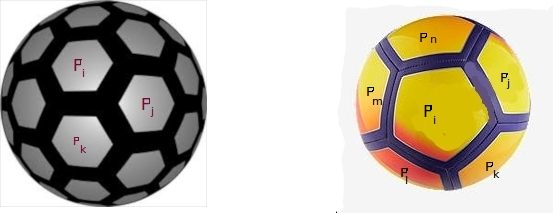
\includegraphics[width=0.6\textwidth]{ball-nike-pitch.jpg}
\caption{}
\end{figure}

Now we present the formal definition of (CS) as derived from Bieri-Eckmann's homological duality \cite{BiEck}, \cite{BS}. When the reader reviews the definition of homology with coefficients in a chain complex \cite{Brown}, then one finds the problem of (CS) amounts to constructing a nontrivial $0$-cycle $\xi \in H_0(\Gamma; \underline{\bZ}_2 \Gamma \otimes \bD)$. Bieri-Eckmann duality says $$H_0(\Gamma; \underline{\bZ}_2 \Gamma \otimes \bD) \approx H^\nu(\Gamma; \underline{\bZ}_2 \Gamma)\approx \underline{\bZ}_2 \otimes_\bZ \textbf{D}\neq 0.$$ Thus we deduce the formal existence of nontrivial $0$-cycles. However our applications will require nontrivial $0$-cycles which satisfy further ``convex" assumptions, c.f. \eqref{cs} below.

The group $\Gamma$ of symmetries flips, rotates, and translates the base cycle $[P]$ throughout the space, and every finite subset $I$ of $\Gamma$ produces a finite chain sum $$\sum_{\gamma\in I} [P].\gamma,$$ with total chain boundary $$\del(\sum_{\gamma\in I} [P].\gamma)=\sum_{\gamma\in I} \del [P].\gamma.$$ \textit{The basic problem of Closing Steinberg is to produce a finite subset $I \subset \Gamma$ for which the boundary of the nontrivial chain sum $\sum_{\gamma\in I} [P].\gamma$ vanishes in the mod $2$ homology group.} The complete definition of Closing Steinberg includes further geometric conditions on the $\Gamma$-translates $F.\Gamma$ of the the closed convex hull $F=conv[P.I]$ of the translates $B.I$. Let $\sT[t], \del \sT[t]$ be a $\Gamma$-invariant excision of $\sT$. Let $[P]$ be a flat-filled relative cycle representing a nonzero generator of $H_{q+1}(\sT[t], \del \sT[t]; \bZ)$.

\begin{dfn}[\textbf{Closing Steinberg}]\label{cs}
A finite subset $I$ of $\Gamma$ successfully Closes Steinberg if: 

\textbf{(i: nontrivial mod $2$)} the chain $\xi=\sum_{\gamma\in I} P.\gamma $ is nonvanishing over $\bZ/2$ coefficients in the chain group $C_{q+1}(\sT[t],\del \sT[t];\bZ/2)$;  

\textbf{(ii: vanishing boundary mod $2$)} the boundary $\del \xi=\sum_{\gamma\in I} \del [P].\gamma $
vanishes over $\bZ/2$-coefficients in the homology group $[\del \xi]=0$ in $H_q(\del \sT[t]; \bZ)$;

\textbf{(iii: well-defined convex hull)} the boundary-chain representing $\del \xi$ is simultaneously visible from an interior point $x$ in $\sT[t]$;

\textbf{(iv: well-separated gates)} there exists a finite-index subgroup $\Gamma' < \Gamma$ such that the chain sum $\uF=\sum_{\gamma \in \Gamma'}F.\gamma$ has nonempty \emph{well-separated gates} precisely equal to the principal orbit $\{P.\gamma ~|~ \gamma\in \Gamma'\}$. 
%the translates $B.\gamma$, per $\gamma\in I$, are geometrically disjoint in $X[t]$.
\end{dfn}

Our definition of Closing Steinberg was inspired by the author's study of \cite{Cremona}. In Cremona's terminology, the problem is to determine a ``relation ideal $\mathscr{R}$" and construct a ``basic polyhedron $P$ whose transforms fill the space", c.f.\cite[pp.290]{Cremona}. 


 %Cremona successfully Closes Steinberg in several cases for $\Gamma=GL(\mathscr{O}_{\sqrt{-d}})$, where $\mathscr{O}_{\sqrt{-d}}$ is the ring of integers of some Euclidean complex quadratic fields. 
The hypotheses (i)--(ii) basically require the chain sum $\xi$ to be nonzero mod $2$. The hypotheses (iii)--(iv) are ``convex" assumptions, and which need be verified for any nonzero chain. The hypothesis of well-separated gates is related to the following fact: the translates $P, P.\gamma$, for $\gamma\in \Gamma$, are either identical or geometrically disjoint in $\sT[t]$ according to Lemma \ref{kl}. However the translates $P, P.\gamma$ may have nontrivial intersection at infinity in the initial Teichmueller space $\sT$. In fact the problem of (CS) is precisly to find such nontrivial intersections at infinity, although again the intersections are disjoint in the interior of $\sT[t]$.

%Moreover the convexity assumptions are nontrivial, and require a new metric on $\sT$. For indeed we should require the metric to be nonpositively curved











%As developed by Ivanov (inspired by Borel-Serre [ref]) we can also identify the dualizing module $\bD$ with the reduced homology of the rational boundary at-infinity: $\bD \simeq \tilde{H}_*(\del_{\infty, rational} T)$. With this observation 

%\subsection{}
%[Curve Complex][Broaddus, duality][Steinberg module]


%(Action on Steinberg Symbols) The curve complex consists of simple closed curves $\gamma$ on $\Sigma$. The free homotopy class $[\gamma]$ corresponds to a conjugacy class in $\pi_1$. Therefore the curve complex consists of a special subset of ``simple" conjugacy classes $[\gamma]$. The algebraic characterization of those conjugacy classes which represent simple curves appears difficult problem [ref]. Obviously the mapping classes $\Gamma$ act by translation on the conjugacy classes, and coincides to the action of $\Gamma$ on $CC$ (simple closed curves). 
%Question: How to symbolically represent the conjugacy classes? Given a faithful linear representation $\rho$ of $\pi$, how to represent conjugacy classes? 
%Problem: Want to formally (CS) on computer. How to find translates of the Steinberg symbol? [Aramayona-Leininger, Birman-Broaddus-Leininger]










%\subsection{Closing Steinberg (CS)}
%The definition of (CS) is a motivated by the standard idea of fundamental domains, \cite[\S 3.5, pp.163]{PR}. Let $(X,d,\sigma)$ be a mm-space, with isometric action $X\times \Gamma \to X$. A \textit{fundamental domain} of $(X,\Gamma)$ is a measurable subset $D\subset X$ satisfying: 

%(FD1) the union of the $\Gamma$-translates covers $X$, so $\cup_{\gamma \in \Gamma} D.\gamma = X$; 

%(FD2) the translates have null intersection $\sigma[D \cap D\gamma]=0$ for every $\gamma\neq id_\Gamma$; and

%(FD3) the measure $\sigma[D]$ equals the volume of the quotient space $X/\Gamma$ with respect to the pushforward measure $p\# \sigma$, where $p: X \to X/ \Gamma$ is the quotient map. 

%The reader should observe that explicit constructions of fundamental domains are nontrivial and frequently impossible. Defining the fundamental domain $D$ is essentially equivalent to specifying all generators and relations in the group $\Gamma$. But imperfect knowledge of $\Gamma$ restricts one's ability to construct such precise fundamental domains. Acknowledging our imperfect \`a priori knowledge of $\Gamma$, we introduced the definition of ``Closing the Steinberg symbol" in [ref]. We abbreviate this subprogram ``(CS)" for ``Closing Steinberg". (CS) is a weaker condition than constructing fundamental domains. Instead (CS) seeks a measurable subset $D$ such that a stronger form of (FD2) is satisfied and such that $\cup_{\gamma \in \Gamma} D.\gamma$ is a simply-connected subdomain of $X$, i.e. the inclusion $\cup_{\gamma \in \Gamma} D.\gamma \subset X$ is a $\Gamma$-equivariant homotopy-equivalence. So (CS) constructs a truncated fundamental-type domain.  Our constructions below construct domains $D=F[t]$ equal to the convex-excision of a compact convex subdomain $F$ of $X$. 

%Explicit constructions of fundamental domains for the action $\sT \times \Gamma \to \sT$ is practically impossible, and requires precise knowledge of generators and relations in $\Gamma$. Acknowledging our imperfect \`a priori knowledge of $\Gamma$, we introduced the definition of ``Closing the Steinberg symbol" in [ref], abbreviated (CS). 


\section{Open Problem: (CS) for Genus 2}
To illustrate our ideas, we now study the case of genus two closed Riemann surface. The duality theory of mapping class groups $\Gamma=MCG(\Sigma_g)$ for genus $g=2$ has been described by \cite{Broaddus2012}. For reference we include the following figure taken from \cite[Fig.10]{Broaddus2012}, see \eqref{br}.%Let $B$ be Broaddus' two-sphere in the curve complex $\sC$. 

\begin{figure}\label{br}
\centering
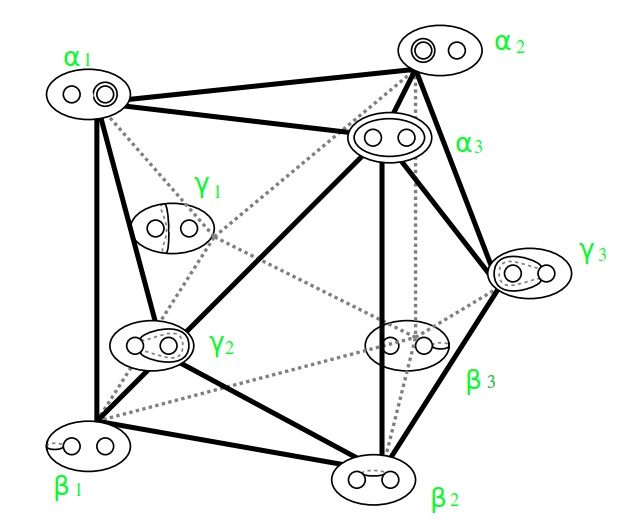
\includegraphics[width=0.6\textwidth]{broaddus-sphere-marked-new.png}
\caption{Homologically nontrivial $2$-sphere in the curve complex $\sC$ of genus $2$ closed surface. Figure adapted from \cite[Fig.10]{Broaddus2012}}
\end{figure}
%Observe $B$ has nine vertices $\alpha_1, \alpha_2, \alpha_3,\beta_1, \beta_2, \beta_3.$ The sets of curves $\{\alpha_1, \alpha_2, \alpha_3\}$ and $\{\alpha_4, \alpha_5, \alpha_6\}$ are pants decompositions. The curves $\beta_1, \beta_2, \beta_3$ are separating curves on $\Sigma$. Then (CS) requires a finite subset $I \subset \Gamma$ such that the chain sum $$SUM [\{\alpha_i.\gamma, ~\beta_j.\gamma |~~i=1,\ldots,6,~~j=1,2,3, ~~\gamma \in I\}] $$ vanishes over $\bZ/2$-coefficients, i.e. such that $$\sum_{\gamma \in I} (\alpha_1.\gamma+\cdots+\alpha_6.\gamma+\beta_1.\gamma+ \beta_2.\gamma+ \beta_3.\gamma )=0 ~~ (mod~ 2).$$ 

%We remark that Broaddus' nine curves do not satisfy the $9g-9$ theorem, i.e. the lengths of Broaddus' curves do not sufficiently discriminate between marked genus two Riemann surfaces. 


%\subsection{Formal Solutions of (CS) in genus two}
The formal problem of (CS) for genus two surfaces has the following symbolic setup. Let $V:=\bZ/2(\sC^0)$ be the abelian topological group consisting of finitely-supported $\bZ/2$-valued functions $f: \sC^0 \to \bZ/2$ on the set of free homotopy classes of simple closed curves on a surface $\Sigma$. Symbolically, we abbreviate such a function $f$ with its support $\alpha+\beta+\ldots$. On the genus two closed surface, consider Broaddus' set of nine curves $\alpha_i, \beta_j, \gamma_k$, $i,j,k \in \{1,2,3\}$, and especially the formal sum $$\sB:= \sum_{i,j,k=1}^{3} \alpha_i+\beta_j+\gamma_k.$$ Now finally we make the problem of (CS) totally explicit: 

\begin{dfn}
A finite subset $I\subset \Gamma$ formally Closes Steinberg for the mapping class group $\Gamma$ of genus two closed surfaces if 
\begin{equation}
\label{bb}
\sum_{\phi\in I} \sum_{\alpha\in \sB}\alpha.\phi=0, ~~mod~2,
\end{equation}
where the zero element $0$ on the right hand side is the zero element in $V$, i.e. the constant zero-valued distribution on $\sC^0$. 
\end{dfn}

Symbolically the ``vanishing mod $2$" of the translates $\sum_{\phi\in I} \sB.\phi$ says there is an \emph{even} number of coincidences between the translated curves $\alpha.\phi$ where $\phi\in I$, $\alpha\in \sB$. 

Remark. Obviously the group structure of $\Gamma$ allows us to restrict ourselves to subsets $I$ containing the identity mapping class $Id\in \Gamma$. 

To illustrate, let the reader observe that a typical element $\phi\in MCG$ will \emph{totally displace} the curves in $\sB$ such that $\sB \cap \sB.\phi=\emptyset$ for almost every $\phi\in MCG$. On the other hand, if $\phi'$ permutes the curves such that $\sB.\phi=\sB$, then $I=\{Id,\phi'\}$ would be a solution of \eqref{bb}. However we consider this solution to be trivial in the following sense: the formal sum $[\sB]+[\sB].\phi'=2[\sB]=0$ is itself vanishing mod $2$. Such trivial solutions are avoided in the case of higher genus closed surfaces as the work of \cite{birman2013finite} demonstrates, i.e. the identity element is the only mapping class which permutes $\sB$. Obviously parabolic type elements $\phi$, i.e. curve stabilizers $\phi\in MCG_\gamma$ satisfy$\sB \cap \sB.\phi \supset \{\gamma\}$. So naturally one is tempted to find formal solutions to (CS) by choosing a suitable sequence of parabolics. 

It is possible that finite subgroups of $\Gamma$ provide convenient solutions $I$ to (CS) in higher genus, as the examples in \cite{Cremona} demonstrate. The structure of finite subgroups in the genus $g=2$ mapping class group is however too limited. Thus we are forced to search out solutions to (CS) directly. While \eqref{bb} provides an explicit symbolic statement of (CS), it remains difficult to actually search for such solutions. The problem is to represent the action of the mapping class group on the simplicial curve complex $\sC$. The curve complex $\sC$ consists of free homotopy classes of simple closed curves $\alpha$ on $\Sigma$. The free homotopy class $[\alpha]$ corresponds to a conjugacy class in $\pi_1$. Therefore the curve complex consists of a special subset of ``simple" conjugacy classes $[\alpha]$. The algebraic characterization of those conjugacy classes which represent simple curves appears difficult problem.

Here we find the question: 

-\emph{How to symbolically compute the $\Gamma$-action $[\alpha] . \phi$ on $\sC$?} 

To answer the above question would permit a brute force search for formal solutions to (CS). We would represent a neighborhood of the identity element in $\Gamma$ and then randomly search for formal solutions by directly evaluating the chain sums $\sum_\phi [\sB].\phi$ and their boundaries $\sum_\phi \del[\sB].\phi$ mod 2.

Another possibility arises though, based on Mark C. Bell's curver program \url{https://curver.readthedocs.io/en/master/index.html}. Our experimentation with curver is however limited by the fact that curver is restricted to surfaces with punctures or marked points, and is not immediately applicable to closed surfaces (although this limitation is possibly the author's own).  

Finally we remark that Professor I.V Nikolaev claims to have established the \emph{linearity} of the mapping class groups of closed surfaces \cite{nikolaev2018mapping}, \cite{nikolaev2001toric}, yet we find the articles rather difficult to understand and implement, being based on some results of $AF$ $C^*$-algebras.


\section{A Naive Possibility}
The following naive possibility arises. Let $\rho:\pi \to GL_N$ be a linear finite-dimensional representation of $\pi:=\pi_1(\Sigma, pt)$ of a pointed closed Riemann surface. Let $N=N_{GL}(\rho)$ be the normalizer of the image of $\rho$ in $GL_N$. Then we find the image $Im(\rho)$ is a normal subgroup of $N$, and we obtain a quotient group $Im(\rho)\backslash N$ with a canonical homomorphism $$\chi_\rho: Im(\rho)\backslash N \to Out(\pi).$$

\begin{prob}
\label{fdrep}
Does there exist a finite-dimensional linear representation $\rho$ of $\pi$ such that the homomorphism $\chi_\rho$ is surjective?
\end{prob}

A solution to Problem \ref{fdrep} would allow an effectively \emph{linear} representation of the elements of $MCG$. The question is whether embedding $\pi$ into a larger matrix group provides a larger class of outer automorphisms to be represented by matrix conjugation.









%\section{}
%We remark that \emph{if} the mapping class group admitted an effective linear representation, then our methods for solving (CS) for arithmetic groups could be extended. For the basic arithmetic group $\Gamma=PGL(\bZ^2)$, a convenient solution to (CS) is given by $$I_0=\{Id, \begin{pmatrix} 1 & 1 \\ 0 & 1 \end{pmatrix}, \begin{pmatrix} 0 & 1 \\ -1 & 2 \end{pmatrix}\}.$$ Thus the chain sum $$\xi:= 
%(\begin{bmatrix} 1 \\ 0 \end{bmatrix} \otimes \begin{bmatrix} 0 \\ 1 \end{bmatrix}) + 
%(\begin{bmatrix} 0 \\ 1 \end{bmatrix} \otimes \begin{bmatrix} 1 \\ 1 \end{bmatrix}) +
%(\begin{bmatrix} 1 \\ 1 \end{bmatrix} \otimes \begin{bmatrix} 1 \\ 0 \end{bmatrix}) $$ represents a nontrivial $0$-cycle $\xi \in H_0(PGL(\bZ^2) , \bZ_2 \otimes \textbf{D})$, where $\textbf{D}$ is the dualizing $\bZ PGL(\bZ^2)$-module $\approx H_1(Proj[\del Q[t]]; \bZ)$. So $\del_0 \xi=0$ where $\del_0$ is the chain boundary operator. The reader can consult \cite[]{martel}. 



%Indeed the problem of (CS) has the following form: we look for subsets $\{\alpha'\}$ of $\sC$ and want nontrivial elements $\phi\in MCG$, $\phi\neq Id$, such that the intersection $\{\alpha'\}' \cap \{\alpha'.\phi\}'$ is nonempty.















%\subsection{Examples: Some Arithmetic Groups}
%We have constructed formal solutions to (CS) for arithmetic groups $\Gamma=G(\bZ)$ in a few low-dimensional cases. These solutions were found using Wolfram MATHEMATICA. For example, the following subsets $I$ are (formal) solutions for the matrix groups $\Gamma=GL(\bZ^2)$, $GL(\bZ^3)$, $Sp(\bZ^4)$, respectively: [insert].

%However we are yet unable to use Wolfram to identify formal solutions to [eqref]. Firstly this is because $MCG$ is not known to admit any linear representations, and secondly because we do not know how to ``encode" simple closed curves and their orbits under mapping class elements. Perhaps Thurston's train-tracks and $PML$ are the natural encoding, although we have not yet pursued this possibility.


\section{Well-Separated Gates: From (CS) To Candidate Spines}
Suppose the user succesfully Closes the Steinberg symbol, i.e. finds a finite subset $I$ of $\Gamma$ satisfying conditions \ref{cs}. Solutions to (CS) allow us to replace $\sT$ and rational excisions $\sT[t] \subset \sT$ with \emph{ a chain sum $\uF$ with \textbf{well-separated gates}}, a term which also appears in item \eqref{cs}(iv) in the definition of (CS). This is a term introduced in \cite[pp.13, \S 5.1]{martel}, and means $\uF=\sum_{i\in I} F_i$ is a countable chain sum of sets $F_i$ where the intersections $G:=F_{ij}:=F_i\cap F_j$ have a well-behaved fixed geometry. In our applications the chain summands $F_i$ are convex excisions of the form $F_i=F[t]$ (see \cite[\S 5.5]{martel}). The idea is next that gated costs (see \cite[\S 5.2]{martel}) are determined by their restrictions to the summands $F_i$, and also by the gates $G\subset F_i$ which are contained in the given summand. Thus we reduce the study of costs on $\sT[t]$ to localized costs defined on the summands $F_i$ and with respect to the gates $G\subset F_i$. This reduces us to the setting of \cite[\S 5.9]{martel} where we studied various repulsion costs on convex excisions. 

If $\uF$ is a chain sum with well-separated gates $\{G\}$, then the singularity locus $\sZ$ naturally decomposes as a chain sum $\sZ=\sum_i \sZ \cap F_i$, and where $\sZ \cap F_i$ is the singularity locus of a restricted semicoupling program, with respect to the restricted cost $c|F_i$. Best results are obtained with costs satisfying Properties (D0)--(D4) and we conjecture that the visibility costs satisfy (D0)--(D4) using the notation of \cite{martel}. Finally using the Reduction to Singularity method of \cite[Theorems 1.4.1-2]{martel}, we naturally construct continuous deformation retracts and which even assemble to global continuous retracts $\sT \leadsto \sZ$. N.B. constructing the retraction is contingent on the user having an effective computable model of $\sT$ available. Generally $\sZ$ has large codimension in $\sT$ depending on so-called Uniform Halfspace Conditions. Symmetries in the excision boundary (and target measure) on $\del \sT[t]$ increases the maximal codimension of $\sZ$ with the possibility of attaining the extreme codimension, even the equivariant spine of $\sT$. Again all the above requires the user have an effective model available. Here there is much to say, but we go no further in this article.

%\section{On Canonical Geometric $E\Gamma$ models.}

%[INCOMPLETE]

%Our thesis \cite{martel} studied the importance of using different models for various $E\Gamma$ classifying spaces. So what is the best model of Teichmueller's space $\sT$? Indeed this article has not yet formally defined the \emph{points} of $\sT$, neither have we defined the action of $\Gamma=MCG(\Sigma)$ on $\sT$. 



%The discovery of models of hyperbolic geometry in the careers of Gauss, Lobachevsky, \etc, is enormous discovery for the human mind. And especially the proper discontinuous actions of $PGL(\bZ^2)$ on the unit two dimensional disk $D^2$. The incredible formula $$z.\begin{pmatrix} a & b // c & d \end{pmatrix}:=(az+b)(cz+d)^{-1}$$ describing the group of Mobius transformations on the complex plane. It is further incredible that the Mobius group acts by conformal transformation (holomorphically) on $z$ (i.e. the above formula has no terms involving $\bar{z}$ in any power series representation). %How to make the action of $PGL(\bZ^2)$ on the disk as 
 





%(?) Observe no triple of Broaddus' curves are related by a Dehn twist, i.e. no relations of the type $\alpha_k=D_{\alpha_i}(\alpha_j)$, where $D_{\alpha_i}$ is a Dehn twist about $\alpha_i$. 
%\begin{lem}
%For every marked surface $X\in \sT_2$, the gradients $\nabla_X \ell_{\alpha_i}$, $\nabla_X \ell_{\beta_j}$ with respect to WP-metric, for $i=1,\ldots,6$, $\beta=1,2,3$ span a three-dimensional convex hull, i.e. the gradients span a four-dimensional subset of $T_X \sT$. 
%\end{lem}
%\begin{proof}
%Wolpert's formula [ref] proves the gradients of cuff lengths of a pants decomposition are linearly independant and almost orthogonal. 
%\end{proof}
%The above formulation of (CS) for Broaddus' two-sphere can be further simplified. Let $\beta_1, \beta_2, \beta_3$ be the three separating curves in Broaddus' two-sphere $B$. 
%\begin{prob}
%Determine finite subsets $I \subset \Gamma$ such that $$\sum_{\gamma \in I} \beta_1.\gamma+\beta_2.\gamma+\beta_3.\gamma =0 , ~~(mod~2).$$ 
%\end{prob}
%A solution to Problem [ref] has the form $$abc+bcd+aef+efd.$$ This requires finding $\phi, \phi' \in \Gamma$ such that $$\phi(a)=a, \phi(b)=e, \phi(c)=f$$ and $$\phi'(a)=d, \phi(b)=b, \phi(c)=c,$$ where $a,b,c,\ldots$ are separating curves.
 

%(punctured torus) Observations: if $\beta$ is a separating curve, then $\Gamma_\beta$ is isomorphic to a direct product $GL(\bZ^2) \times GL(\bZ^2)$, where we recall $MCG_+(\Sigma_{1,1}) \approx GL(\bZ^2)$. 

%[Insert: Wolpert, gradient computations]

%\section{Convexity and $9g-9$ Theorem}
%Observe that Lemma [ref].(ii) implies $T[t]$ coincides with the closed visibly-convex hull of $\del T[t]$ in $T[t]$. 
%The reader may compare this observation with Wolpert's theorem that $\bar{T}$ is the geodesic convex hull of marked maximally-noded Riemann surfaces. [ref?] 

%The augmented Teichmuller space $\bar{\sT}$ with $WP$-geometry has certain analogy to Voronoi's cone $V$ of positive-semidefinite quadratic states $q: \bR^N \to \bR_{\geq 0}$, $q(v):={}^t v Q v$ where $Q$ is a positive semidefinite symmetric operator and $v\in \bR^N$. Krein-Milman's theorem [ref] implies $\bar{V}$ is the closed convex hull of rank-one quadratic forms, specifically $\ell(v)^2$, where $\ell \in \bR^{N *}-\{0\}$ is a nontrivial linear form. [Ref]. 

%Analogous to Voronoi's state space [ref], there are infinitely-many faces meeting at the extreme points $\sE$ of $\bar{T}$. Compare [ref: Gunnell's appendix, Stein, Modular forms]. The visibility relation $V$ on $T[t] \times \del T[t]$ allows the application of Krein-Milman's theorem to the nonconvex excision model $T[t]$. 
  




%Let $\sT$ be Teichmueller space equipped with WP-metric $d=d_{WP}$. If $f: \sT \to \bR$ is a function, then $\nabla f$ denotes the gradient of $f$ defined with respect to $WP$-metric. 
%\begin{dfn}
%Let $X$ be a hyperbolic surface. We say a collection $\{\alpha_0, \alpha_1, \ldots \}$ of simple closed curves is affinely-independant if the gradients $\{\nabla \ell_{\alpha_0} X - \nabla \ell_{\alpha_i} X \}_{i\geq 1}$ are a linearly-independant subset of $T_X \sT$. 
%\end{dfn}

%We say the collection $\{\alpha_0, \alpha_1, \ldots \}$ has affine-dimension $d$ if $span\{\nabla \ell_{\alpha_0} X - \nabla \ell_{\alpha_i} X\}_{i\geq 1}$ is $d$-dimensional.





%Various spines have been conjectured. Notably W.Thurston [ref] proposed those surfaces whose systoles are filling as a spine. However this characterization does not appear to have the correct codimension in $\sT$, and his proposed flow is discontinuous. Recently Ji, Ji/Wolpert [ref] constructed a codimension-two deformation retract for all $g\geq 2$. Following an argument of S.Wolpert and H. Parlier, [Ji: Proposition 4.3] proves the set $S''$ consisting of $X\in \sT_g$ with the properties  that $\#sys_1(X)\geq 3$ and there exists $\alpha, \beta \in sys_1(X)$ such that $|\alpha \cap \beta |\geq 1$ is a codimension-two deformation retract for $g\geq 2$. Harer [ref: Harer] obtained explicit spines for punctured mapping class groups $MCG(\Sigma_{g,p})$ where $p\geq 1$ is the number of punctures. This ``punctured" case is considerably easier than the closed case $p=0$. 




%[Below: Incorrect]
%This leads us to conjecture that the set of all genus $g$ hyperbolic surfaces $X$ whose systoles $sys_1(X)$ has affine-dimension $\geq 2g-1$ forms a $MCG$-equivariant spine of $\sT(\Sigma_g)$. Thus we propose
%$$\sW_g:=\{X\in \sT_g |~\dim(span\{\nabla \ell_\alpha X | ~\alpha\in sys_1(X) \})\geq 2g\}$$ is a closed $MCG$-equivariant deformation retract of $\sT_g$. The above subset $\sW_g$ evidently has the correct codimension in $\sT$, as required by the fact that $$vcd(MGC_g)=6g-6-(2g-1)=4g-5,$$ and it remains to prove $\sW_g \hookrightarrow \sT_g$ is an equivariant deformation-retract. Alternatively we can characterize $\sW$ as consisting of hyperbolic surfaces $X$ whose systoles $sys_1(X)$ contains at least $2g$ disjoint simple closed curves. 
%The set $S''$ is evidently different than our set $\sW_g$ for $g\geq 2$. 
%In analogy with Soul\'e-Ash's well-rounded retract, we seek an elementary continuous flow which deforms $\sT$ onto $\sW$.  
%Thus we are proposing that the set of hyperbolic surfaces $X$ whose systoles $sys_1(X)$ are disjoint is a spine for $\sT$. Since the maximum number of disjoint simple closed curves on a genus $g$ surface is $2g-1$, we can equivalently characterize the spine as those surfaces admitting a ``systolic pants decomposition". 






%\section{}
%The purpose of this note is to highlight an elementary problem which we call ``Closing the Steinberg symbol", and to describe its application to constructing minimal $MCG$-invariant spines of Teichmuller's space $\sT$. We begin with the genus $g=2$ oriented closed surface. The starting point is Broaddus' $2$-sphere $B$ desribed in [ref]. This $2$-sphere is a homologically nontrivial sphere in the simplicial curve complex $\sC=\sC(\Sigma_2)$. Considered as a $\bZ MCG$-module, the reduced integral homology groups $\tilde{H}_2(\sC;\bZ)$ represents the dualizing module $D$ of $MCG$. Broaddus' $2$-sphere $B$ and its translates by $MCG$ generate the $\underline{\bZ/2\bZ} MCG$-module $D\otimes \bZ/2\bZ$. Now we imagine $B$ as the ``panel", and seek some translates $B, B.\phi_1, B.\phi_2, \ldots$ of panels whose chain sum $B+ B.\phi_1+ B.\phi_2+ \cdots$. The problem is motivated by stitching a football from panels. [ref].

%\section{Teichmueller and Weil-Peterson metrics}
%The present note constructs an explicit spine for the mapping class group $\Gamma=MCG(\Sigma_g)$ of a closed Riemann surface of genus $g\geq 2$. We construct a closed Lipschitz subvariety $\underline{Z}=Z_{J+1}$ of the Teichmueller space $T=Teich(\Sigma_g)$ such that $\underline{Z} \hookrightarrow T$ is a $\Gamma$-equivariant continuous deformation retract and where $\dim(\underline{Z})=vcd(\Gamma)$. In otherwords $\underline{Z}$ is a minimal-dimension $E\Gamma$ classifying space. Our construction depends on special finite subsets $I \subset \Gamma$ of mapping class elements which successfully ``Close the Steinberg symbol", see Definition [ref] below. 

%The constructions of equivariant deformations of Teichmueller space have typically depended directly on systole-type functionals, which are Morse-like functions, c.f. [Ji], [Ji-Wolpert], [Bavard]. However these methods only achieve codimension $\leq 2$ retracts, and are rather limited. There is famous preprint of Thurston \cite{} which contains major error and constructs a discontinuous retract. Our thesis develops a new general method for constructing souls and spines, based on Kantorovich's singularity functor $Z$, which is a contravariant functor $Z: 2^{Y} \to 2^{X}$ defined $Z=Z(v, \sigma, \tau)$ where $v:X\times Y \to \bR$ is cost function, $(X,\sigma)$ is a source mm-space and $(Y,\tau)$ is a target mm-space. 
%We apply our general method to the source space $X=T[t]$, target $Y=\del T[t]$, with visibility cost $v$, where $T[t]$ is a convex-excision of Teichmueller's space $T=Teich(\Sigma_g)$. 








%Observation: if $\{P_i\}$ is a tessalation of $X$ with vertices at finite positions in $X$, then the tiling is not necessarily aspherical, and the chain sum $\sum P_i$ will not be homotopy-equivalent to $X$. Indeed, the existence of vertices at finite positions allows the possibility that $\sum P_i$ admits nontrivial (finite) coverings. However if all vertices exist ``at-infinity", then there exists no finite lifts (and no finite coverings). 

%Thurston Straightening: an ideal simplex admits no self-mappings of degree $\geq 2$. Analogously a relative simplex $(B, \del B)$ in $(X[t], \del X[t])$ admits no self-mapping of degree $\geq 2$. 
%Lemma: If $X[t]$ is excision model as above, then $X[t] \times \del X[t]$ does not admit any self-mappings of degree $\geq 2$.   


%[Rephrase: find finite subgroup of MCG such that action on curve-complex CC(S) has orbit which `Closes Steinberg'?] Sample the Connoly-Wosneiscki paper, with explicit finite subgroups -- any accidents? 

%For case of genus two, we observe that a Dehn twist $D_\gamma$ about a vertex $\gamma$ of $P$ will fix the link of $\gamma$ pointwise, and $D_\gamma$ will therefore translate exactly three vertices $\delta_1, \delta_2, \delta_3$ of $P$ to three new vertices $ \delta'_1, \delta'_2, \delta'_3$ of $P.D_\gamma$. The chain sum $P+P.D_\gamma$ therefore has total of six vertices, after reduction modulo 2, namely $\delta_1, \delta_2, \delta_3$, $ \delta'_1, \delta'_2, \delta'_3$. Likewise, a translate of $P.D_\gamma$ by another Dehn twist $D_{\gamma'}$ [Incomplete]

%Elementary observation: we can readily identify a finite subgroup $\approx \bZ /2 \times \bZ/2$ of the genus two mapping class group. But this finite (order four) subgroup has an orbit which does not `CS'.














\printbibliography[title={References}]
\end{document}
